% la-01-labasics.tex

\documentclass[xcolor=dvipsnames]{beamer}
\usepackage{teachbeamer}

\title{Matrix Basics}
\subtitle{{\CourseNumber}, BCIT}

\author{\CourseName}

\date{September 10, 2018}

\begin{document}

\begin{frame}
  \titlepage
\end{frame}

\begin{frame}
  \frametitle{Matrix Definition}
  A \alert{matrix} is a tabular arrangement of real numbers. 
  \begin{equation}
    \label{eq:oathaemo}
    A=\left[\begin{array}{cccc}
    a_{11}&a_{12}&\cdots{}&a_{1n} \\
          a_{21}&\ddots{}&& \\
          \vdots{}&&&\vdots \\
          a_{m1}&&\cdots{}&a_{mn}
  \end{array}\right]
\end{equation}
The number of rows is $m$, the number of columns is $n$. $m\times{}n$
is called the \alert{dimension} or \alert{size} of the matrix.
\end{frame}

\begin{frame}
  \frametitle{Matrix Addition}
We can define operations on matrices just like we define operations on
numbers. For example, we can add an $m\times{}n$ matrix to another one
as follows,
\begin{equation}
  \label{eq:ahloongi}
  \left[\begin{array}{cccc}
    a_{11}&a_{12}&\cdots{}&a_{1n} \\
          a_{21}&\ddots{}&& \\
          \vdots{}&&&\vdots \\
          a_{m1}&&\cdots{}&a_{mn}
  \end{array}\right]+\left[
\begin{array}{cccc}
    b_{11}&b_{12}&\cdots{}&b_{1n} \\
          b_{21}&\ddots{}&& \\
          \vdots{}&&&\vdots \\
          b_{m1}&&\cdots{}&b_{mn}
  \end{array}\right]=\notag
\end{equation}
\begin{equation}
  \label{eq:fohghoaw}
\left[
\begin{array}{cccc}
    a_{11}+b_{11}&a_{12}+b_{12}&\cdots{}&a_{1n}+b_{1n} \\
          a_{21}+b_{21}&\ddots{}&& \\
          \vdots{}&&&\vdots \\
          a_{m1}+b_{m1}&&\cdots{}&a_{mn}+b_{mn}
  \end{array}\right]\notag
\end{equation}
\end{frame}

\begin{frame}
  \frametitle{Matrix Addition}
  \beispiel{Adding and Subtracting Matrices}
  \begin{equation}
    \label{eq:pahleuza}
    \left[
      \begin{array}{cc}
        1 & -2 \\
        -3 & -1 
      \end{array}\right]+\left[
      \begin{array}{cc}
        3 & -3 \\
        4 & 1
      \end{array}\right]=\left[
      \begin{array}{cc}
        4 & -5 \\
        1 & 0
      \end{array}\right]\notag
  \end{equation}
  \begin{equation}
    \label{eq:euquolux}
    \left[
      \begin{array}{cc}
        5 & -6 \\
        -2 & 2 
      \end{array}\right]-\left[
      \begin{array}{cc}
        -6 & 5 \\
        0 & 7
      \end{array}\right]=\left[
      \begin{array}{cc}
        11 & -11 \\
        -2 & -5
      \end{array}\right]\notag
  \end{equation}
\end{frame}

\begin{frame}
  \frametitle{Matrix Scalar Multiplication}
Next, we define what it means to multiply a matrix by a \alert{scalar}, i.e.\
a real number (NOT a matrix). 
\begin{equation}
  \label{eq:theishie}
  k\cdot\left[\begin{array}{cccc}
    a_{11}&a_{12}&\cdots{}&a_{1n} \\
          a_{21}&\ddots{}&& \\
          \vdots{}&&&\vdots \\
          a_{m1}&&\cdots{}&a_{mn}
  \end{array}\right]=\left[\begin{array}{cccc}
    ka_{11}&ka_{12}&\cdots{}&ka_{1n} \\
          ka_{21}&\ddots{}&& \\
          \vdots{}&&&\vdots \\
          ka_{m1}&&\cdots{}&ka_{mn}
  \end{array}\right]\notag
\end{equation}
\end{frame}

\begin{frame}
  \frametitle{Matrix Scalar Multiplication}
  \beispiel{Multiplying a Matrix by a Scalar}
  \begin{equation}
    \label{eq:quooroaw}
    2\cdot\left[
      \begin{array}{cc}
        -5 & -3 \\
        -7 & 8 
      \end{array}\right]=\left[
      \begin{array}{cc}
        -10 & -6 \\
        -14 & 16
      \end{array}\right]\notag
  \end{equation}
  \begin{equation}
    \label{eq:xaexoopi}
    -\frac{1}{3}\cdot\left[
      \begin{array}{cc}
        -1 & -3 \\
        -7 & 1 
      \end{array}\right]=\left[
      \begin{array}{cc}
        \frac{1}{3} & 1 \\
        \frac{7}{3} & -\frac{1}{3}
      \end{array}\right]\notag
  \end{equation}
\end{frame}

\begin{frame}
  \frametitle{Matrix Transpose}
  The columns of a \alert{transpose} $A^{\intercal}$ are the rows of the
  matrix $A$. The rows of a transpose $A^{\intercal}$ are the columns
  of the matrix $A$.
  \begin{equation}
    \label{eq:chuiruth}
        A=\left[\begin{array}{cccc}
    a_{11}&a_{12}&\cdots{}&a_{1n} \\
          a_{21}&\ddots{}&& \\
          \vdots{}&&&\vdots \\
          a_{m1}&&\cdots{}&a_{mn}
  \end{array}\right]\notag
  \end{equation}
  \begin{equation}
    \label{eq:aetheini}
        A^{\intercal}=\left[\begin{array}{cccc}
    a_{11}&a_{21}&\cdots{}&a_{n1} \\
          a_{12}&\ddots{}&& \\
          \vdots{}&&&\vdots \\
          a_{1m}&&\cdots{}&a_{nm}
  \end{array}\right]\notag
  \end{equation}
\end{frame}

\begin{frame}
  \frametitle{Matrix Transpose}
  \beispiel{Transposing a Matrix}
  \begin{equation}
    \label{eq:ujaesuch}
    \left[
      \begin{array}{ccc}
        -1 & 2 & 1 \\
        7 & -2 & -1 \\
        0 & 6 & 6 \\
        7 & 6 & 4
      \end{array}\right]^{\intercal}=\left[
      \begin{array}{cccc}
        -1 & 7 & 0 & 7 \\
        2 & -2 & 6 & 6 \\
        1 & -1 & 6 & 4
      \end{array}\right]
  \end{equation}
\end{frame}

\begin{frame}
  \frametitle{Matrix Product}
Finally, we define \alert{matrix multiplication}. You can multiply an
$m\times{}j$ matrix by a $j\times{}n$ matrix, which will give you an
$m\times{}n$ matrix.
\begin{equation}
  \label{eq:orahpahn}
  \left[\begin{array}{cccc}
    a_{11}&a_{12}&\cdots{}&a_{1j} \\
          a_{21}&\ddots{}&& \\
          \vdots{}&&&\vdots \\
          a_{m1}&&\cdots{}&a_{mj}
  \end{array}\right]\cdot
\left[\begin{array}{cccc}
    b_{11}&b_{12}&\cdots{}&b_{1n} \\
          b_{21}&\ddots{}&& \\
          \vdots{}&&&\vdots \\
          b_{j1}&&\cdots{}&b_{jn}
  \end{array}\right]=\notag
\end{equation}
\begin{equation}
  \label{eq:raipuboi}
  \left[\begin{array}{cccc}
    c_{11}&c_{12}&\cdots{}&c_{1n} \\
          c_{21}&\ddots{}&& \\
          \vdots{}&&&\vdots \\
          c_{m1}&&\cdots{}&c_{mn}
  \end{array}\right]\notag
\end{equation}
where $c_{ik}=a_{i1}b_{1k}+a_{i2}b_{2k}+\ldots+a_{ij}b_{jk}$.
\end{frame}

\begin{frame}
  \frametitle{Matrix Product}
  Notice that $c_{ik}$ is the product of the $i$-th row vector of $A$
  and the $k$-th column vector of $B$. The dot product of two vectors
  $\vec{v}$ and $\vec{w}$ is defined to be
  $\vec{v}\,^{\intercal}\cdot\vec{w}$.

\medskip

  \beispiel{Multiplying Matrices}
  \begin{equation}
    \label{eq:eroogaju}
    \left[
      \begin{array}{cc}
        -1 & 5 \\
        10 & 8 
      \end{array}\right]\cdot\left[
      \begin{array}{cc}
        -3 & -8 \\
        7 & 0
      \end{array}\right]=\left[
      \begin{array}{cc}
        38 & 8 \\
        26 & -80
      \end{array}\right]\notag
  \end{equation}
\end{frame}

\begin{frame}
  \frametitle{Matrix Product}
  {\ubung} Consider
  \begin{equation}
    \label{eq:tiequooh}
    A=\left[
      \begin{array}{cc}
        0 & -1 \\
        3 & 2
      \end{array}\right]\hspace{.5in}B=\left[
      \begin{array}{cc}
        1 & -2 \\
        2 & 1
      \end{array}\right]
  \end{equation}
Find $A\cdot{}B$ as well as $B\cdot{}A$ and determine whether matrix
multiplication is commutative.
\end{frame}

\begin{frame}
  \frametitle{Laws for Matrix Arithmetic}
  All the usual laws of arithmetic hold for matrix arithmetic, for
  example $A(B+C)=AB+AC$ or $c(AB)=(cA)B=A(cB)$. There are two major
  exceptions:
  \begin{enumerate}
  \item The order of factors cannot be interchanged: $AB=BA$ is
    generally not true
  \item $AB=0$ does not imply that one of the matrices is the zero
    matrix, for example
    \begin{equation}
      \label{eq:equaewoi}
      \left[
        \begin{array}{cc}
          2 & 3 \\
          -4 & -6
        \end{array}\right]\cdot\left[
        \begin{array}{cc}
          3 & -6 \\
          -2 & 4
        \end{array}\right]=\left[
        \begin{array}{cc}
          0 & 0 \\
          0 & 0
        \end{array}\right]
    \end{equation}
  \end{enumerate}
\end{frame}

\begin{frame}
  \frametitle{Identity Matrix}
The \alert{identity matrix} $I$ with dimension $m\times{}m$ is a square matrix
such that for all $m\times{}m$ matrices $A$ it is true that
\begin{equation}
  \label{eq:aivaitoa}
  A\cdot{}I=I\cdot{}A=A
\end{equation}
An identity matrix always has all $1$'s in the diagonal and all $0$'s
elsewhere.
\begin{equation}
  \label{eq:ubaisula}
  I=\left[
    \begin{array}{cccc}
      1 & 0 & \ldots & 0 \\
      0 & 1 & \ldots & 0 \\
      \vdots & & \ddots & \vdots \\
      0 & \ldots & 0 & 1
    \end{array}\right]
\end{equation}
\end{frame}

\begin{frame}
  \frametitle{Matrix Inverse}
The \alert{inverse matrix} $A^{-1}$ of a square matrix $A$ is the
matrix for which
\begin{equation}
  \label{eq:quoovain}
  A\cdot{}A^{-1}=A^{-1}\cdot{}A=I
\end{equation}
Not all matrices have an inverse. Finding the inverse of a
$m\times{}m$ matrix is equivalent to solving a system of $m\cdot{}m$
equations with $m\cdot{}m$ variables. For example, the inverse of the
matrix
\begin{equation}
  \label{eq:iiphiese}
  A=\left[
    \begin{array}{cc}
      a & b \\
      c & d
    \end{array}\right]\hspace{.25in}\mbox{ is }\hspace{.25in}A^{-1}=\frac{1}{ad-bc}\left[
    \begin{array}{cc}
      d & -b \\
      -c & a
    \end{array}\right]
\end{equation}
\end{frame}

\begin{frame}
  \frametitle{Matrix Determinant}
  Considering the last slide, it is evident that a matrix has an
  inverse if and only if $ad-bc\neq{}0$. Such a matrix is called
  \alert{invertible}. If $ad-bc=0$ then the matrix is \alert{singular}
  and has no inverse (find some examples). It turns out that the
  number $ad-bc$ is so special for $2\times{}2$ matrices that it gets
  its own name: it is the \alert{determinant} of the matrix. On the
  next slide, I will define the determinant of any square matrix using
  an inductive procedure.
\end{frame}

\begin{frame}
  \frametitle{Matrix Determinant}
  \begin{itemize}
  \item The determinant of a $1\times{}1$ matrix $A$ is
    $\det(A)=a_{11}$.
  \item The determinant of a $m\times{}m$ matrix with $m>1$ is
    $\det(A)=c$. 
  \end{itemize}
  Calculate $c$ by picking an arbitrary row, for example the $i$-th
  row. Then
  \begin{equation}
    \label{eq:queiyesh}
    c=\sum_{j=1}^{m}(-1)^{i+j}a_{ij}\det(A_{ij})
  \end{equation}
  $A_{ij}$ is the matrix that results when you delete the $i$-th row
  and the $j$-th column from $A$.
\end{frame}

\begin{frame}
  \frametitle{Rules for Determinants}
  \begin{enumerate}
  \item The determinant of a matrix equals the determinant of its
    transpose.
  \item If a matrix has a row or a column of zeroes, the determinant
    is zero.
  \item Interchanging two rows (or columns) changes the sign of the
    determinant.
  \item The determinant of an upper triangular matrix is the product
    of its diagonal entries.
  \end{enumerate}
  It follows from rule 3 that the determinant of a matrix, where two
  rows or columns are equal, is zero (why?). 
\end{frame}

\begin{frame}
  \frametitle{Adjugate Matrix}
The \alert{adjugate matrix} of a matrix $A$ has as its elements the
real numbers $b_{ji}$ (note the switched indices) with
\begin{equation}
  \label{eq:quesieha}
  b_{ji}=(-1)^{i+j}\det(A_{ij})
\end{equation}
where $A_{ij}$ is defined on a previous slide. Consequently,
\begin{equation}
  \label{eq:iegoowae}
  \det(A)\cdot{}I=\mbox{adj}(A)\cdot{}A
\end{equation}
for all square matrices $A$. This is true because the diagonal entries
of $\mbox{adj}(A)\cdot{}A$ correspond to the definition of $\det(A)$.
The non-diagonal entries correspond to the definition of
$\det(\hat{A})$, where $\hat{A}$ is a matrix with two columns of $A$
repeated.
\end{frame}

\begin{frame}
  \frametitle{Calculating the Adjugate Matrix}
  \begin{description}
  \item[Step 1: Determinants of Minor Square Matrices] For each
    element of the matrix $a_{ij}$, delete the $i$-th row and the
    $j$-th column and calculate the determinant of the matrix $A_{ij}$
    that is left over. Put that determinant in a new matrix in
    $a_{ij}$'s place.
  \item[Step 2: Multiply by Checkerboard Matrix] Multiply each element
    of the result matrix in step 1 by each element of the checkerboard
    matrix (see next slide). (This way of multiplying matrices is
    called Hadamard multiplication as opposed to matrix
    multiplication.)
  \item[Step 3: Transpose] Now transpose the result matrix of step 2
    in order to calculate the adjugate matrix.
  \end{description}
\end{frame}

\begin{frame}
  \frametitle{Calculating the Adjugate Matrix Example}
  \alert{Step 1}
  \begin{equation}
    \label{eq:oyingiej}
    \left[
      \begin{array}{ccc}
        4 & 1 & -3 \\
        3 & 0 & 1 \\
        8 & -1 & 2
      \end{array}\right]\longrightarrow\left[
      \begin{array}{ccc}
        1 & -2 & -3 \\
        -1 & 32 & -12 \\
        1 & 13 & -3
      \end{array}\right]\notag
  \end{equation}
  \alert{Step 2}
  \begin{equation}
    \label{eq:ewezohhu}
    \left[
      \begin{array}{ccc}
        1 & -2 & -3 \\
        -1 & 32 & -12 \\
        1 & 13 & -3
      \end{array}\right]\longrightarrow\left[
      \begin{array}{ccc}
        1 & 2 & -3 \\
        1 & 32 & 12 \\
        1 & -13 & -3
      \end{array}\right]\notag
  \end{equation}
  \begin{equation}
    \label{eq:ooyegeuk}
\mbox{Checkerboard Matrix: }\left[
      \begin{array}{ccc}
        1 & -1 & 1 \\
        -1 & 1 & -1 \\
        1 & -1 & 1
      \end{array}\right]\mbox{ or }\left[
      \begin{array}{ccc}
        + & - & + \\
        - & + & - \\
        + & - & +
      \end{array}\right]\notag
  \end{equation}
  \alert{Step 3}
  \begin{equation}
    \label{eq:oazefako}
    \left[
      \begin{array}{ccc}
        1 & 2 & -3 \\
        1 & 32 & 12 \\
        1 & -13 & -3
      \end{array}\right]\longrightarrow\left[
      \begin{array}{ccc}
        1 & 1 & 1 \\
        2 & 32 & -13 \\
        -3 & -12 & -3
      \end{array}\right]\notag
  \end{equation}
\end{frame}

\begin{frame}
  \frametitle{Finding Inverse Using Adjugate}
  Right-multiply equation~(\ref{eq:iegoowae}) by $A^{-1}$ to see that
  \begin{equation}
    \label{eq:foomochu}
    A^{-1}=\frac{1}{\det(A)}\mbox{adj}(A)
  \end{equation}
  For example, the adjugate of
  \begin{equation}
    \label{eq:soojohdi}
    \left[
      \begin{array}{ccc}
        0 & -1 & 4 \\
        3 & 2 & 0 \\
        4 & 3 & 1 
      \end{array}\right]\mbox{ is }\left[
      \begin{array}{ccc}
        2 & -3 & 1 \\
        13 & -16 & -4 \\
        -8 & 12 & 3 
\end{array}\right]^{\intercal}
  \end{equation}
  Therefore, the inverse is
  \begin{equation}
    \label{eq:fiaphaid}
    \frac{1}{7}\cdot\left[
      \begin{array}{ccc}
        2 & 13 & -8 \\
        -3 & -16 & 12 \\
        1 & -4 & 3 
      \end{array}\right]
  \end{equation}
\end{frame}

\begin{frame}
  \frametitle{Matrix Determinants Exercises}  
  {\ubung} Consider
  \begin{equation}
    \label{eq:aengixoh}
    B=\left[
      \begin{array}{cc}
        1 & 0 \\
        3 & -2 
      \end{array}\right]
  \end{equation}
  Calculate $B^{-1}$ and show that $B\cdot{}B^{-1}=I$.

  \medskip

  {\ubung} Consider
  \begin{equation}
    \label{eq:eecheipo}
    D=\left[
      \begin{array}{ccc}
        0 & -1 & 4 \\
        3 & 2 & 0 \\
        4 & 3 & -1 
      \end{array}\right]
  \end{equation}
Calculate $\det(D)$. Then use software to calculate the inverse of
$D$. What do you notice about $\det(D)\cdot{}D^{-1}$?
\end{frame}

\begin{frame}
  \frametitle{Using Determinants to find Areas}
  The absolute value of the determinant of a 2x2 matrix $A$ is the
  area of the following parallelogram:
  \begin{enumerate}
  \item One vertex of the parallelogram is at the origin. Call it $O$.
  \item Two vertices are at $U=(a_{11},a_{12})$ and
    $V=(a_{21},a_{22})$.
  \item The final vertex is at $W=(a_{11}+a_{21},a_{12}+a_{22})$.
  \end{enumerate}
  A proof without words is on the next slide. Alternatively, you can
  watch a video with the proof here:
  \texttt{https://youtu.be/n-S63\_goDFg}.
\end{frame}

\begin{frame}
  \frametitle{Using Determinants to find Areas}
    \begin{figure}[h]
    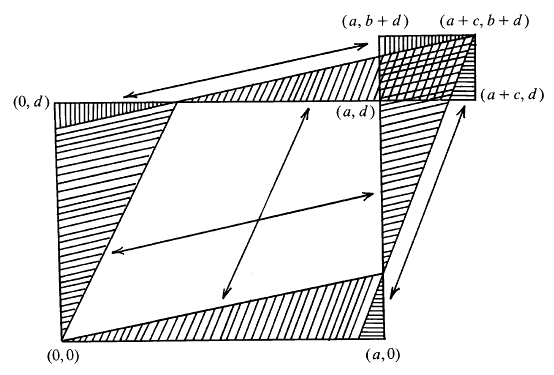
\includegraphics[scale=.5]{./diagrams/pardet1.png}
  \end{figure}
\end{frame}

\begin{frame}
  \frametitle{Using Determinants to find Areas}
  The principle can be generalized to higher dimensions. The volume of
  a parallelepiped is the absolute value of the determinant of the
  three vectors spanning it put side by side in a matrix.

  \beispiel{Parallelepiped} Find the oriented volume of the
  parallelepiped built on
  $a_{1}=(2,1,0)^{\intercal},a_{2}=(0,3,11)^{\intercal},a_{3}=(1,2,7)^{\intercal}$
  in $\mathbb{R}^{3}$.
  Solution: the volume is
  \begin{equation}
    \label{eq:waixaimi}
    \left\vert\det\left(\left[
        \begin{array}{ccc}
          2 & 1 & 0 \\
          0 & 3 & 11 \\
          1 & 2 & 7
        \end{array}\right]\right)\right\vert=9
  \end{equation}
\end{frame}

\begin{frame}
  \frametitle{Using Determinants to find Areas}
  If the figure based on parallelograms has dimension $k\leq{}n$ use
  the Gramian matrix. Its determinant is the square of the area,
  volume, etc.\ of the figure based on parallelograms.

  \beispiel{Gramian Matrix} Find the area of the parallelogram built
  on $a=(1,−1,2)^{\intercal},b=(2,0,3)^{\intercal}$. Solution: the Gram
  determinant is
  \begin{equation}
    \label{eq:ohgaiheo}
    \det\left(\left[
        \begin{array}{cc}
          6 & 8 \\
          8 & 13
        \end{array}\right]\right)=14
  \end{equation}
Hence the area is $\sqrt{14}$.
% http://www.maths.manchester.ac.uk/~lwalker/MATH10000/project-04-part2.pdf
\end{frame}

\begin{frame}
  \frametitle{Area Exercise}
  {\ubung} Find the area of the triangle with vertices
  $(1,-4),(6,-6),(3,2)$.

  \medskip

  Solution: Move the vertex $(1,-4)$ to the origin. This puts the
  other two vertices at $(5,-2)$ and $(2,6)$. Calculate the
  determinant of
  \begin{equation}
    \label{eq:shuajohs}
    \det\left(\left[
      \begin{array}{cc}
        5 & -2 \\
        2 & 6
      \end{array}\right]\right)=34
  \end{equation}
The area of the triangle is half of the area of the parallelogram. The
answer is 17. 
\end{frame}

\begin{frame}
  \frametitle{End of Lesson}
Next Lesson: Linear Equations
\end{frame}

\end{document}

